%%%%%%%%%%%%%%%%%%%%%%%%%%%%%%%%%%%%%%%%%%%%%%%%%%%%%%%%%%%%%%%%%%%%%%%%%%%%%%%%
%2345678901234567890123456789012345678901234567890123456789012345678901234567890
%        1         2         3         4         5         6         7         8

\documentclass[letterpaper, 11 pt, conference]{ieeeconf}  % Comment this line out
                                                          % if you need a4paper
%\documentclass[a4paper, 10pt, conference]{ieeeconf}      % Use this line for a4
                                                          % paper

\IEEEoverridecommandlockouts                              % This command is only
                                                          % needed if you want to
                                                          % use the \thanks command
\overrideIEEEmargins
% See the \addtolength command later in the file to balance the column lengths
% on the last page of the document

\usepackage{amsmath}
\usepackage{booktabs}
\usepackage{graphicx}
\usepackage{url}


% The following packages can be found on http:\\www.ctan.org
%\usepackage{graphics} % for pdf, bitmapped graphics files
%\usepackage{epsfig} % for postscript graphics files
%\usepackage{mathptmx} % assumes new font selection scheme installed
%\usepackage{times} % assumes new font selection scheme installed
%\usepackage{amsmath} % assumes amsmath package installed
%\usepackage{amssymb}  % assumes amsmath package installed

\title{\LARGE \bf
Report on ``Attitude Determination and Control System Design for a 6U Cubesat for Proximity Operations and Rendezvous" (Franquiz et al)
}

\author{Nathaniel Guy% <-this % stops a space
\thanks{This report is a final project assignment for AA 528, Spacecraft Dynamics and Control, for the '15 Winter quarter at the University of Washington.}
\thanks{N. Guy is a graduate student in the William E. Boeing Department of Aeronautics \& Astronautics, University of Washington, Seattle, WA 98195, USA.
        {\tt\small natguy@uw.edu}}%
}

\begin{document}

\maketitle
\thispagestyle{empty}
\pagestyle{empty}

%%%%%%%%%%%%%%%%%%%%%%%%%%%%%%%%%%%%%%%%%%%%%%%%%%%%%%%%%%%%%%%%%%%%%%%%%%%%%%%%
\begin{abstract}

In this report, I provide a summary, analysis, and critique of the paper ``Attitude Determination and Control System Design for a 6U Cubesat for Proximity Operations and Rendezvous" by Franquiz et al. \cite{franquiz}. This paper presents the design of an ADCS system for a small cubesat, first constraining the problem by presenting mission requirements and formulas for environmental disturbances. The paper then develops two control techniques which are meant to achieve the mission objectives while mitigating these disturbances. I discuss the basic problem that this paper attempts to solve, including how it is framed and how relevant equations are formulated. I also replicate many of their simulations and data analyses, to the extent possible. Finally, I conclude with a critique of the paper's approach to the problem.

\end{abstract}

%%%%%%%%%%%%%%%%%%%%%%%%%%%%%%%%%%%%%%%%%%%%%%%%%%%%%%%%%%%%%%%%%%%%%%%%%%%%%%%%
\section{INTRODUCTION}

\subsection{Paper Goal and Context}

The goal of the reviewed paper is to present and justify a proposed design for the attitude determination and control subsystem (ADCS) for a 6U cubesat towards the completion of a mission called ARAPAIMA. ARAPAIMA, or "Application for Resident space object Automated Proximity Analysis and IMAging," is a mission concept at Embry-Riddle Aeronautical University that is used primarily for astronautics instruction and practice for students, and which may, at some point in the future, develop into an full operational mission. The mission sets as its goal the ability to image and to manipulate the orbits of non-cooperative resident space objects, and this paper, as research related to ARAPAIMA, proposes an ADCS to accomplish the primary goals of orbital approach, pointing, and close-proximity maneuvering.

\subsection{Paper Approach}

This paper first sets about characterizing the mission objectives, vehicle actuators, sensors, and dynamics, and environmental disturbance models, both internal and external. These requirements motivate the development of a controller, which is described in some detail, and followed by numerical simulations of the controller in use. The paper finishes with a discussion of future work and concluding remarks.

%%%%%%%%%%%%%%%%%%%%%%%%%%%%%%%%%%%%%%%%%%%%%%%%%%%%%%%%%%%%%%%%%%%%%%%%%%%%%%%%
\section{SENSING, ACTUATION, DYNAMICS, AND DISTURBANCE MODELS}

\subsection{Vehicle Sensors}

The authors begin by describing their sensor suite on the cubesat. The cubesat is equipped with an infrared camera, a miniature laser rangefinder, a visible light monochrome camera, an IMU with an angular rate gyro and an accelerometer, a startracker, magnetometer sensors, photodiode sunsensors, and an onboard GPS module. (In short, this vehicle seems to be equipped with nearly every attitude sensor the authors could think of!) The placement of the vehicle's external-facing sensors is shown in Fig.~\ref{fig:sensor_placement}.

\subsection{Vehicle Actuators}

The authors continue by describing the vehicle's on-board propulsion system, which consists of a difluoroethane warm gas propulsion system with 16 RCS thrusters, set up in pairs, each capable of producing a maximum of 25 mN of thrust. The placement of the vehicle's RCS thrusters is shown in Fig.~\ref{fig:rcs_placement}.

As an aside, 1,1-difluorethane is a somewhat unconventional choice for a satellite propellant; I can only find one other mention in literature of it being proposed for use \cite{bogdan}. Cold gas N$_{2}$ thrusters are more common for small-scale attitude control in this sort of scenario, but warm gas propellant does achieve higher specific impulse than cold gas propellant, in the 105 to 250 second range \cite{rpe}, which could explain this choice.

The paper actually goes into depth justifying their choice of gas thrusters only, as opposed to the common combination of gas thrusters and reaction wheels. They discuss a study they performed to compare propellant use for 1) a model which uses reaction wheels for torque control, and then uses gas thrusters to offload the momentum of the reaction wheels and 2) a model which uses gas thrusters solely to provide control torques. Their evaluations showed that the gas thruster-only system still achieved acceptable pointing accuracy, with similar propellant use as the reaction wheel/thruster combination, so for greater simplicity they elected to use gas thrusters only.

This conclusion seemed suspect to me, since reaction wheels are generally used as more precise attitude control mechanism than gas thrusters, and I wasn't sure if they could achieve the degree of accuracy they desired with gas thrusters alone, so I did some of the simulations myself using their data. The moment of inertia and exact total disturbance moment wasn't given, but I was able to infer the latter from taking an approximate integral of plots within the paper. (I also guessed the specific impulse of the warm gas propellant system.) The code is included with this report.

This produced a predicted single-orbit propellant usage for RCS-only of 0.324g. This is lower than the paper's prediction of 1g for this task, but it seems like a fair approximation if you take into account imprecisions in my guesses, overshoot, throttle coarseness, and other controller-related overhead.

\subsection{Vehicle Dynamics}

The authors used standard, unit quaternion-based rigid-body dynamics to model the dynamics of the satellite, subject to external and internal disturbance torques and forces. This produced forces and moments as shown below:

\[
F_{b} = m(\dot{V_{b}} + \omega \times V_{b}) + F_{d} + F_{cmd}
\]

\[
M_{b} = J \dot{\omega} + \omega \times (J \omega) + M_{d} + M_{cmd}
\]

The quaternion kinematic equation is expressed as follows:

\[
\dot{\bar{q}}=\frac{1}{2}\left[
\begin{array}{cccc}
 0 & -\omega _x & -\omega _y & -\omega _z \\
 \omega _x & 0 & \omega _z & -\omega _y \\
 \omega _y & -\omega _z & 0 & \omega _x \\
 \omega _z & \omega _y & -\omega _x & 0
\end{array}
\right]\bar{q}
\]

These three equations represent the full dynamics of the model.

\subsection{Vehicle Disturbance Models}

Several external and internal disturbances are modeled in order to predict their effect on the cubesat. The external models include aerodynamic drag torques:

\[
T_{aero} = \frac{1}{2} \rho V_{\infty}^{2} C_{m} Sl
\]

Magnetic residual moment:

\[
T_{rmm} = m_{rmm} \times B_{E}
\]

Gravity gradient torques:

\[
M_{gg} = \frac{2\mu}{|r|^{3}} (\hat{r}) \times J\hat{r}
\]

Solar radiation pressure torques:

\[
M_{srp} = \frac{\Phi f_{s} S_{s} (1+\xi)l_{s}}{c}
\]

These models are consistent with the standard models \cite{smad}.

Internal disturbance models are given for solar panel release dynamics, modeled as a spring-mass damper:

\[
M_{p} = J_{p} \ddot{\theta}_{p} + b \dot{\theta}_{p} + k \theta_{p}
\]

And for propellant slosh:

\begin{multline*}
M_{sl} = -(J_{x,0} + m_{s,0l} h_{0}^{2})\theta_{sl} - \sum^{n} m_{sl,n} h_{sl,n} (\ddot{x}_{sl,n} + H_{sl,n} \theta_{sl,0}) \\
+ g \sum^{n} m_{sl,n} x_{sl,n}
\end{multline*}

(The equation above represents x-axis slosh model only.)

The total effect of disturbance torques, as simulated through the duration of one orbit, is shown in Fig.~\ref{fig:dist_torques}.

\begin{figure}
  \centering
  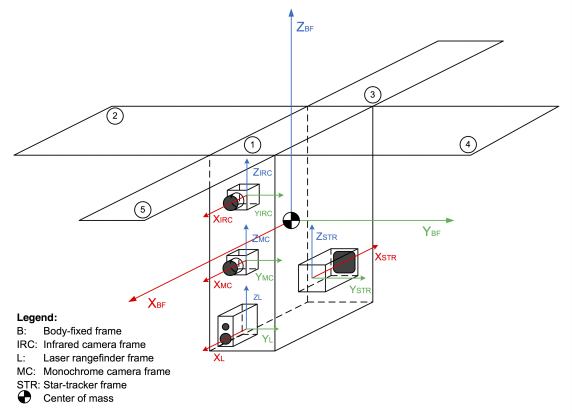
\includegraphics[width=\linewidth]{sensor_placement}
  \caption{Placement of external-facing sensors on the cubesat body.}
  \label{fig:sensor_placement}
\end{figure}

\begin{figure}
  \centering
  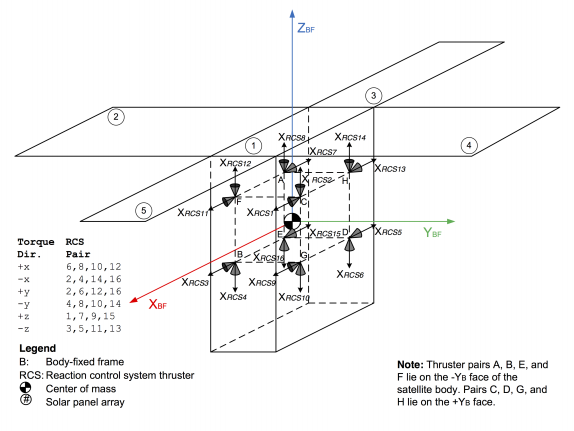
\includegraphics[width=\linewidth]{rcs_placement}
  \caption{Placement of warm gas RCS thruster pairs on the cubesat body.}
  \label{fig:rcs_placement}
\end{figure}


\begin{figure}
  \centering
  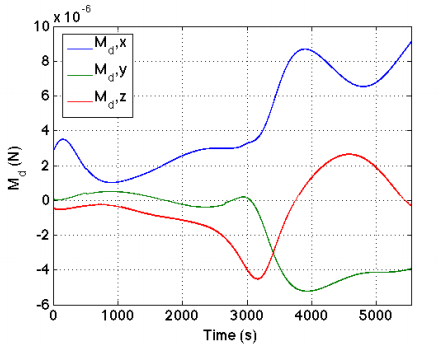
\includegraphics[width=\linewidth]{total_moment_on_satellite}
  \caption{Total effect of disturbance torques over the duration of one orbit.}
  \label{fig:dist_torques}
\end{figure}

%%%%%%%%%%%%%%%%%%%%%%%%%%%%%%%%%%%%%%%%%%%%%%%%%%%%%%%%%%%%%%%%%%%%%%%%%%%%%%%%
\section{CONTROLLER FORMULATION AND SIMULATIONS}

In this paper, the authors develop two control laws to work in conjunction, with a switching scheme to transition between the two.

\subsection{Eigenaxis Control}

The first control law the authors develop is a linear quaternion feedback regulator, based on eigenaxis rotations and analogous to a PD controller via the following control law:

\[
M_{cmd} = -\omega \times J \omega - K_{d} \omega - K_{p} \bar{q}_{e}
\]

I simulated this model for control, with arbitrary, simplified gains and an arbitrary initial state. The PD controller behaves exceptionally. You can see my plots in Fig.~\ref{fig:pdControllerBeta} and Fig.~\ref{fig:pdControllerOmega}, and my code is provided as a supplement.

\begin{figure}
  \centering
  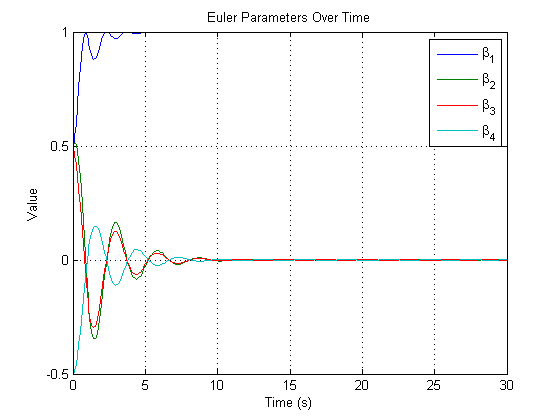
\includegraphics[width=\linewidth]{pdControllerBeta}
  \caption{Quaternion component values with simulated PD controller.}
  \label{fig:pdControllerBeta}
\end{figure}

\begin{figure}
  \centering
  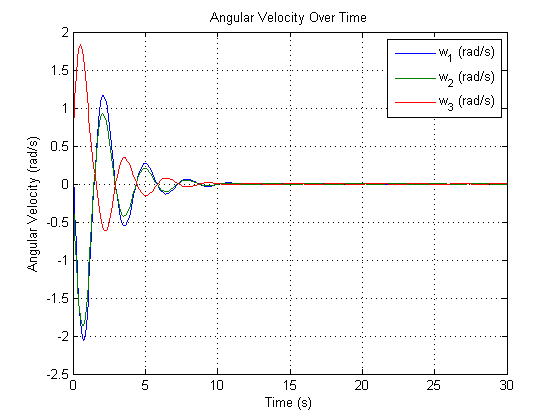
\includegraphics[width=\linewidth]{pdControllerOmega}
  \caption{Angular velocity component values with simulated PD controller.}
  \label{fig:pdControllerOmega}
\end{figure}

\subsection{PID Control}

To combat the steady-state error, the authors then introduced a PID controller about each axis, to be used for high-accuracy imaging modes:

\[
M_{cmd} = - \left[ K_{p} + \frac{K_{i}}{s} + K_{d}s \right] q_{e_{v}}
\]

However, the PID controller cannot be used exclusively, as high integral gains, while useful for correcting steady-state error, are insufficient for large-angle maneuvers, as they increase the settling time dramatically and are very sensitive to the magnitude of the error. For this reason, they employ a bump conditioning algorithm to switch smoothly between the two techniques, and compare it with results from a gain scheduling algorithm to achieve the same task. The results of this comparison can be seen in Fig.~\ref{fig:bc_gs}. The authors of the paper prepared a single-orbit simulation model to simulate this behavior in the presence of the aforementioned disturbance torques. They provide detailed analysis to show that bump conditioning improves overshoot at the controller switch point, and adding gain scheduling improves this even further.

\begin{figure}
  \centering
  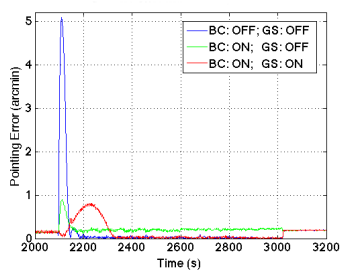
\includegraphics[width=\linewidth]{bc_gs}
  \caption{Bump conditioning and gain scheduling performance comparison.}
  \label{fig:bc_gs}
\end{figure}

\subsection{Future Work}

The authors wrap up their discussion of their work with some proposals for future investigations, followed by some concluding remarks. They suggest that model fidelity needs to be improved, and the algorithms need to be discretized and moved onto the embedded computer in the cubesat. They also give a brief discussion of the issue of noise, which is not explicitly addressed in their model.

%%%%%%%%%%%%%%%%%%%%%%%%%%%%%%%%%%%%%%%%%%%%%%%%%%%%%%%%%%%%%%%%%%%%%%%%%%%%%%%%
\section{CRITIQUE}

I will first discuss what I found pleasing about this paper. I found it to be very readable, and quite generous with its technical data. They went into good detail with their simulation results, and their plots were informative. The approach was a simple one, but plausible, and their discussion of the hardware went into greater detail than many theoretical simulation papers I have seen.


with extremely easy-to-follow diagrams and adequate explanations (or helpful citations) for all of the methods used. Their simulation campaign was aggressive and convincing, with large dispersions and a large introduced delay. I found their conclusion promising, if not wholly convincing.

I did, however, have some issues issues with the content of this paper. Their simulation campaign was very static and not wholly convincing; there appeared to be no stochastic element introduced, and a Monte Carlo simulation with ranges on each disturbance torque would have been a more convincing argument for the robustness of their control. As it currently stands, there is little support for a robustness guarantee on the system, as the gains do not seem to be calculated via an optimal scheme--they appear to be tuned by hand. While the authors do give a brief discussion towards the end of robustness to noise, they only empirically demonstrate that their PID controller is able to counteract a small amount of sensor noise. They also implicitly assume a fully observable system, which may be true when the entire sensor suite is in use, but due to pointing and power-related constraints, it is very likely than not all sensors may be in use at the same time. As they point out, it does seem that their method could benefit from the application of an extended Kalman filter.

Another issue to which they refer in their discussion of future work is that this model is completely continuous, and they have not even begun to analyze its performance on a digital system with delay. This analysis will be necessary for a convincing argument of actual adequacy of the algorithm used.

Though a surprising amount of technical data was given this paper, a few items necessary for data reproduction were missing, including moment of inertia and solar panel surface measurements. They also never discussed constraints on RCS torque except that the thrust is discretized from 0 to 100 by modulating pulse duration; however, I suspect that there may be other constraints, such as power generation conditions and propellant lifetime. 

All in all, I found this paper to be an interesting and educational discussion of a theoretical attitude control problem. The approach is a bit simple and may be able to benefit from the application of more advanced control mechanisms, and more work is needed to prove the viability of the algorithm proposed in the paper, but the results seem promising.

%%%%%%%%%%%%%%%%%%%%%%%%%%%%%%%%%%%%%%%%%%%%%%%%%%%%%%%%%%%%%%%%%%%%%%%%%%%%%%%%

\begin{thebibliography}{99}

\bibitem{franquiz}
F. J. Franquiz, P. Edwards, B. Udrea, M. V. Nayak, and T. Pueschl, Attitude Determination and Control System Design for a 6U CubeSat for Proximity Operations and Rendezvous, {\it AIAA/AAS Astrodynamics Specialist Conference}, 2014.

\bibitem{bogdan}
B. U. Vissidus, "A Cooperative Multi-Satellite Mission for Controlled Active Debris Removal from Low Earth Orbit", {\it IEEE Aerospace 2015}, 2015.

\bibitem{rpe}
G. P. Sutton, O. Biblarz, {\it Rocket Propulsion Elements}, John Wiley \& Sons, Inc., 2010.

\bibitem{smad}
J. Wetz, W. Larson, {\it Space Mission Analysis and Design, 3rd Edition}, Space Technology Library, 1999.

\end{thebibliography}

\end{document}
